\documentclass[lang=cn,newtx,12pt,scheme=chinese]{elegantbook}
\usepackage{setspace}
\renewcommand{\baselinestretch}{2} 

\title{基于语音表型特征的情绪识别系统}
\subtitle{系统使用说明书}

\author{山东省精神卫生中心}
%\institute{}
\date{2024年7月1日}
\version{1.0}
%\bioinfo{自定义}{信息}

%\extrainfo{注意:本模板自 2023 年 1 月 1 日开始,不再更新和维护!}

\setcounter{tocdepth}{3}

%\logo{logo-blue.png}
\cover{cover.jpg}

% 本文档命令
\usepackage{array}
\newcommand{\ccr}[1]{\makecell{{\color{#1}\rule{1cm}{1cm}}}}

% 修改标题页的橙色带
\definecolor{customcolor}{RGB}{32,178,170}
\colorlet{coverlinecolor}{customcolor}
\usepackage{cprotect}

\addbibresource[location=local]{reference.bib} % 参考文献,不要删除

\begin{document}

\maketitle
\frontmatter

\tableofcontents

\mainmatter

\chapter{引言}
\section{编写目的}

本文档为使用说明文档,为软件的使用与维护提供信息基础。

\section{使用对象}

本文档的使用对象主要为产品测试与使用人员。

\section{软件范围}

本产品面向需要进行语音表型特征研究的科研人员,软件提供语音表型特征和情绪识别的功能。

\chapter{软件概述}

为了便于研究人员获取更多的标准化研究数据,自动化提取语音表型特征,所以开发了此软件。

本软件使用Python 3.10进行开发,使用Web浏览器作为GUI界面。软件使用librosa语音分析库实现语音特征的分析和提取,使用matplotlib和seaborn库实现了图表的绘制功能。

另外,软件集成了语音情绪识别模型,可以实现六种情绪的识别。

\section{软件基本信息}

\begin{tabular}{|r|l|r|l|}
  \hline
 软件全称	& 语音表型特征提取和情绪识别系统 & 版本号 & 1.0 \\
  \hline
软件简称  & 语音情绪识别 & 软件分类 & 应用软件\\
  \hline
\end{tabular}


\section{软件功能和技术特点}

\subsection{硬件环境}

开发:华为MateBook,Intel i5处理器,16GB内存,512GB固态硬盘。

运行:华为MateBook,Intel i5处理器,16GB内存,512GB固态硬盘;或macbook pro, 支持M1, M2, M3处理器,16GB内存,512GB固态硬盘;


\subsection{软件环境}

开发:Windows 10系统; Python 3.10版本;VS Code开发工具;

运行:Windows 10系统或MacOS系统,需要安装Python运行环境; Python 3.10;


\subsection{编程语言}

Python 3.10

\subsection{主要功能和技术特点}

\subsubsection{开发目的}

语音特征可以作为诸多疾病的诊断辅助依据,以及用于情绪的识别,针对科研人员在进行语音表型研究过程中,设备操作复杂和特征提取流程繁琐的问题,采用音频采集和特征提取自动化的设计思路,开发了该语音表型特征提取系统软件,可以提取语音的共165个特征值,然后进行情绪的识别。

\subsubsection{面向领域}

医疗大数据分析领域

\subsubsection{主要功能}

1、样本设置。自定义样本基本信息,基本信息会附加到数据文件命名中,方便用户区分样本数据。

2、音频录制。基于麦克风等音频源,进行音频文件的录制,并按自定义文件命名保存为WAV音频文件。

3、音频分析。基于librosa语音库,提取音频文件的MFCC、harmonic、percussive等特征值,并将时序数据、频域数据、频谱数据绘制成图表。

4、情绪识别。基于语音情绪识别模型,针对录制的语音数据进行情绪识别,支持识别“生气”, “厌恶”, “恐惧”, “高兴”, “中性”, “伤心”共6种情绪。


\chapter{使用说明}

\section{使用流程说明}

本软件使用流程主要包括4个步骤。

\begin{enumerate}
  \item 样本设置
  \item 音频录制
  \item 音频分析
  \item 情绪识别
\end{enumerate}

\subsection{系统运行}

点击系统运行程序后,系统会在系统本地启动一个web服务器,然后自动在系统浏览器中新开一个窗口页面,并打开系统的默认首页。首页地址为: http://localhost:8501  或 http://192.168.0.1:8501 。


\subsection{样本设置}

自定义样本基本信息,基本信息会附加到数据文件命名中,方便用户区分样本数据。样本设置的界面如图\ref{fig1}所示。

\begin{figure}
	\label{fig1}
	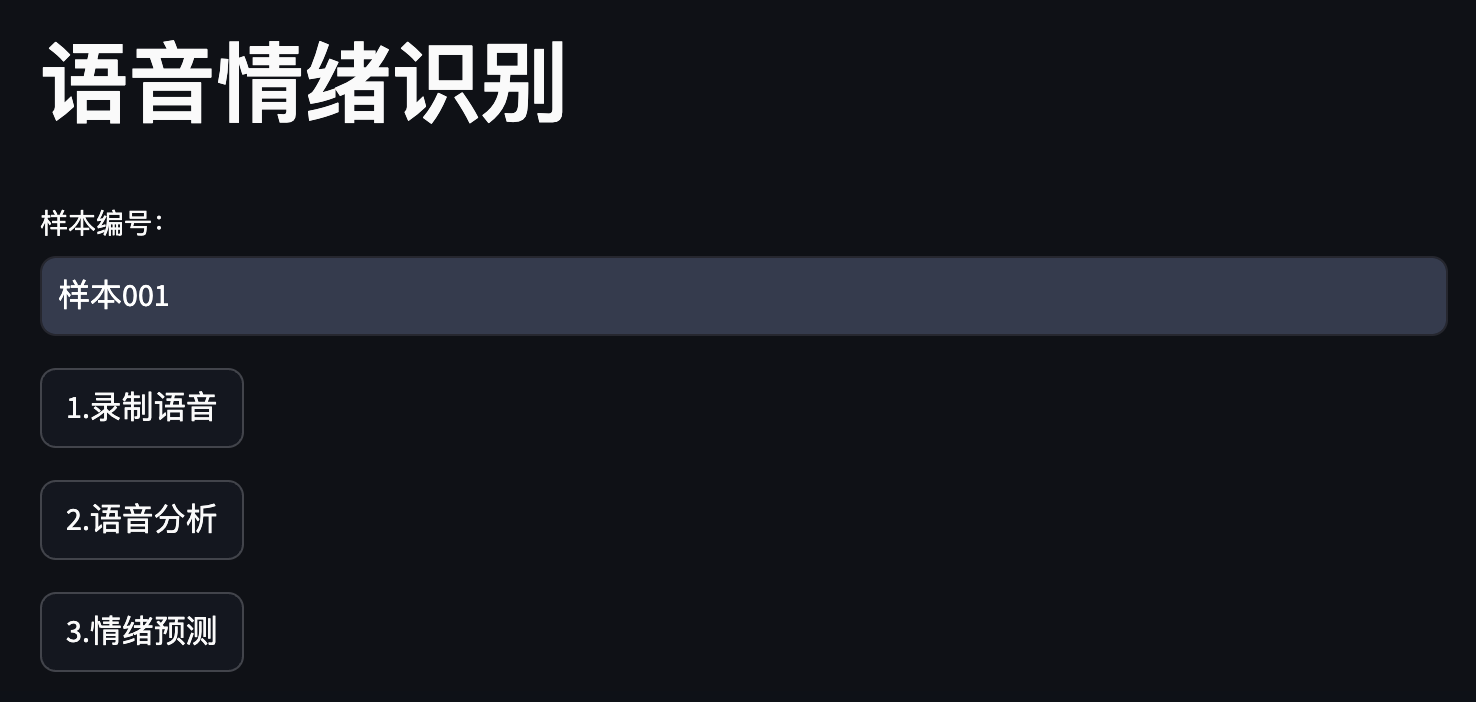
\includegraphics[width=\textwidth]{image/截图1.png}
	\caption{样本编号设置界面}
\end{figure}

\subsection{音频录制}

设置样本编号后,可以点击“1.录制语音”按钮,系统会使用本地机器自带的麦克风等音频输入源设备进行录制,录制过程中,系统会给出“正在录音中”的提示,系统默认会录制30秒的音频数据。界面如图\ref{fig2}所示。

\begin{figure}
	\label{fig2}
	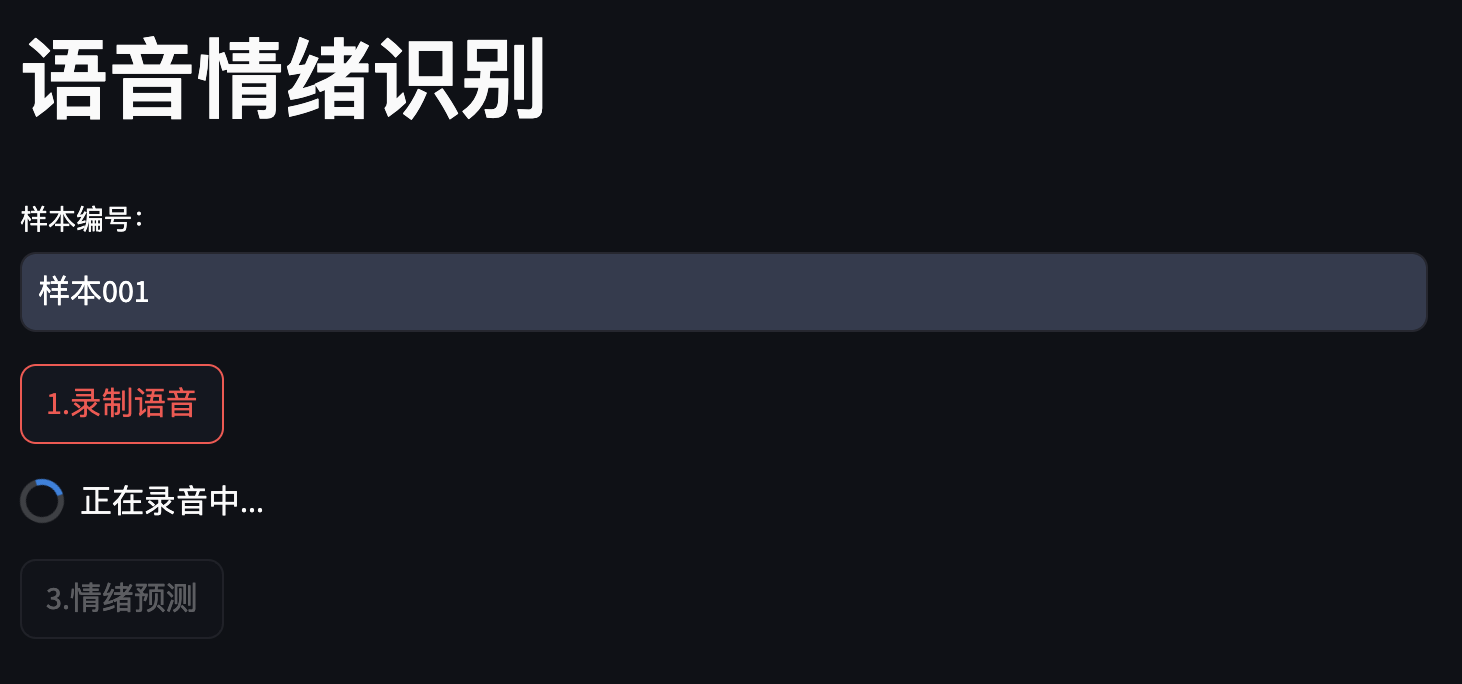
\includegraphics[width=\textwidth]{image/截图2.png}
	\caption{音频录制界面}
\end{figure}

\subsection{音频播放}

等待录音结束后,系统会提示录制完成,并显示一个音频播放器,用户可以使用播放器回放当前样本录制的音频内容,系统操作界面如图\ref{fig3}所示。

\begin{figure}
	\label{fig3}
	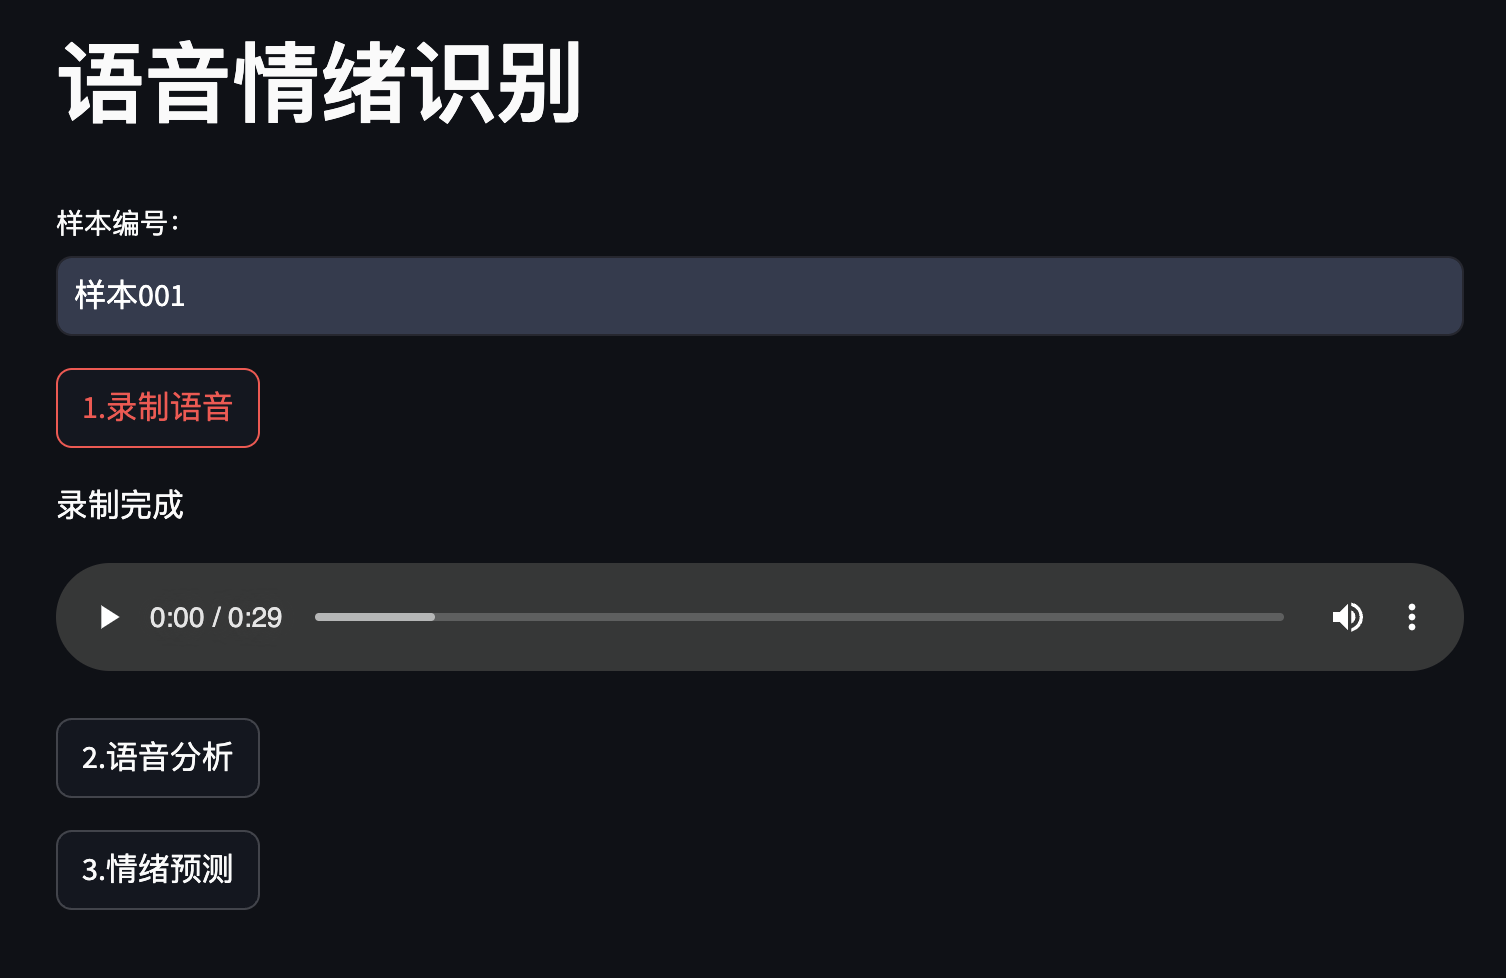
\includegraphics[width=\textwidth]{image/截图3.png}
	\caption{音频播放界面}
\end{figure}

\subsection{音频分析}

音频录制完成后,可以点击语音分析按钮进行当前音频数据的分析,分析结果会分别按时序数据、频域数据、频谱数据三种种类用图表的形式展示出来,如图\ref{fig4}所示。

\begin{figure}
	\label{fig4}
	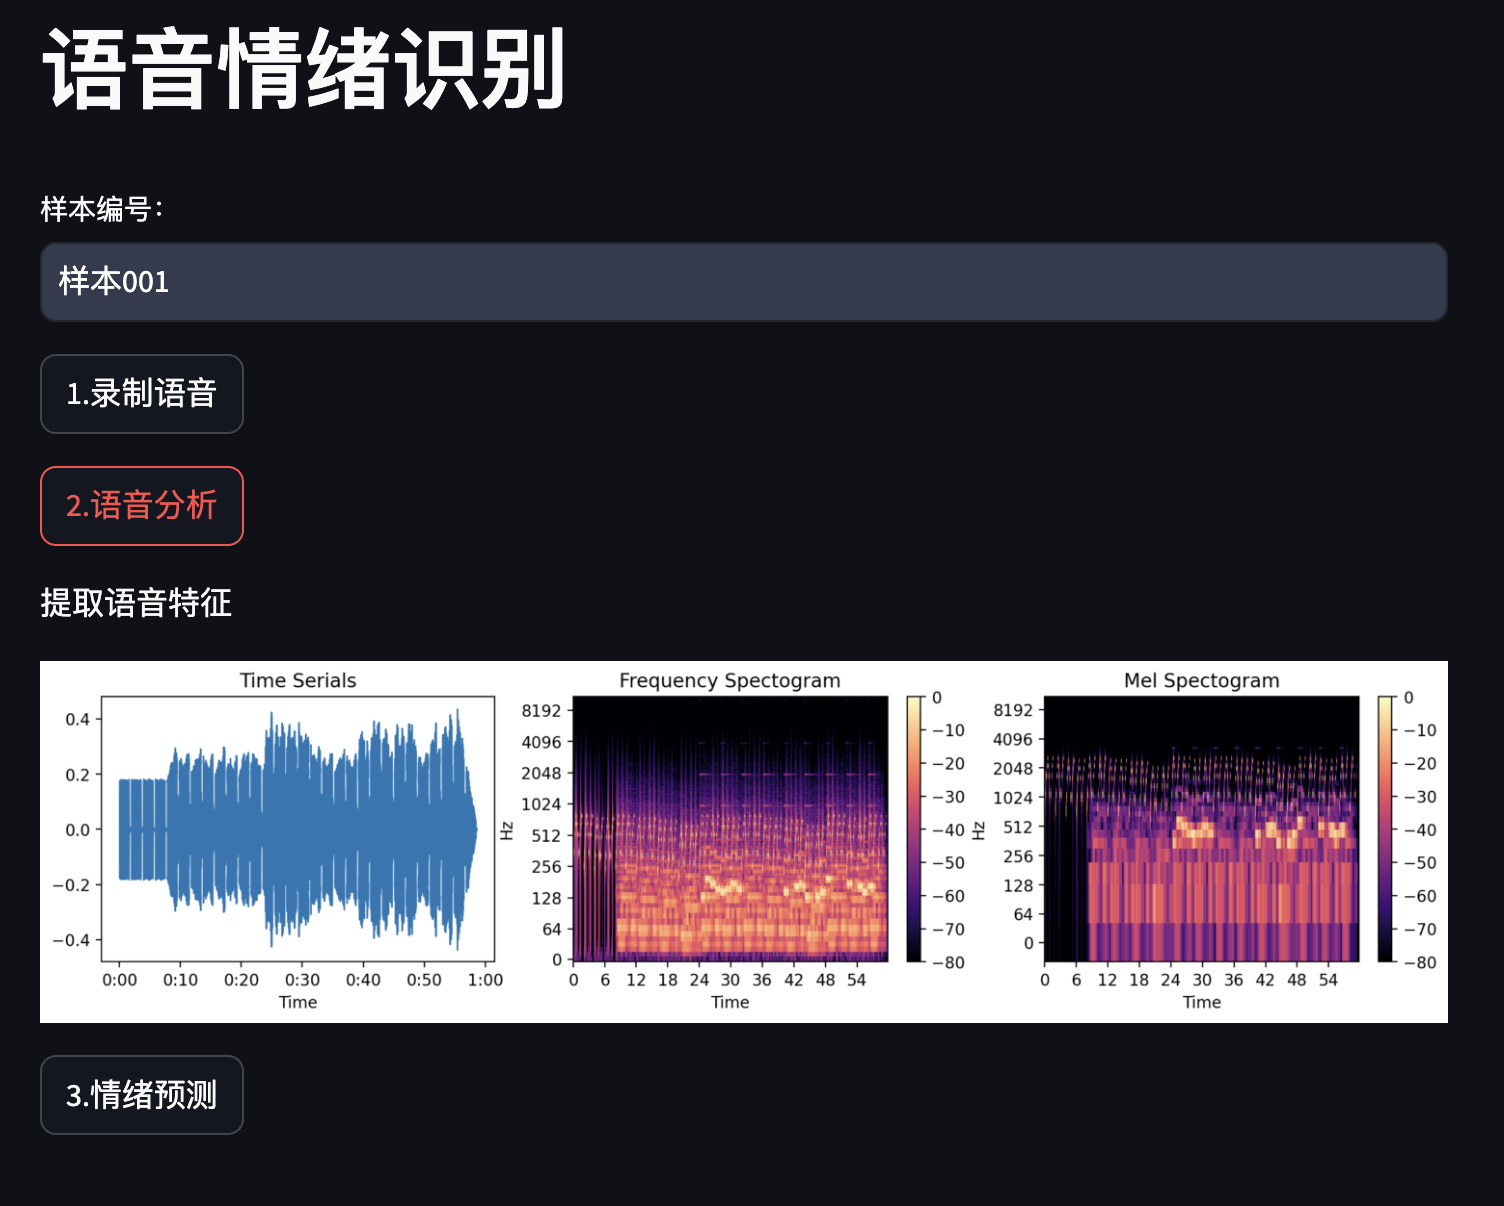
\includegraphics[width=\textwidth]{image/截图4.png}
	\caption{音频分析图表}
\end{figure}

\subsection{情绪识别}

点击情绪预测按扭,系统会调用情绪识别模型,针对当前的样本音频分析结果进行情绪的识别,并显示出预测结果,如图\ref{fig5}所示。

\begin{figure}
	\label{fig5}
	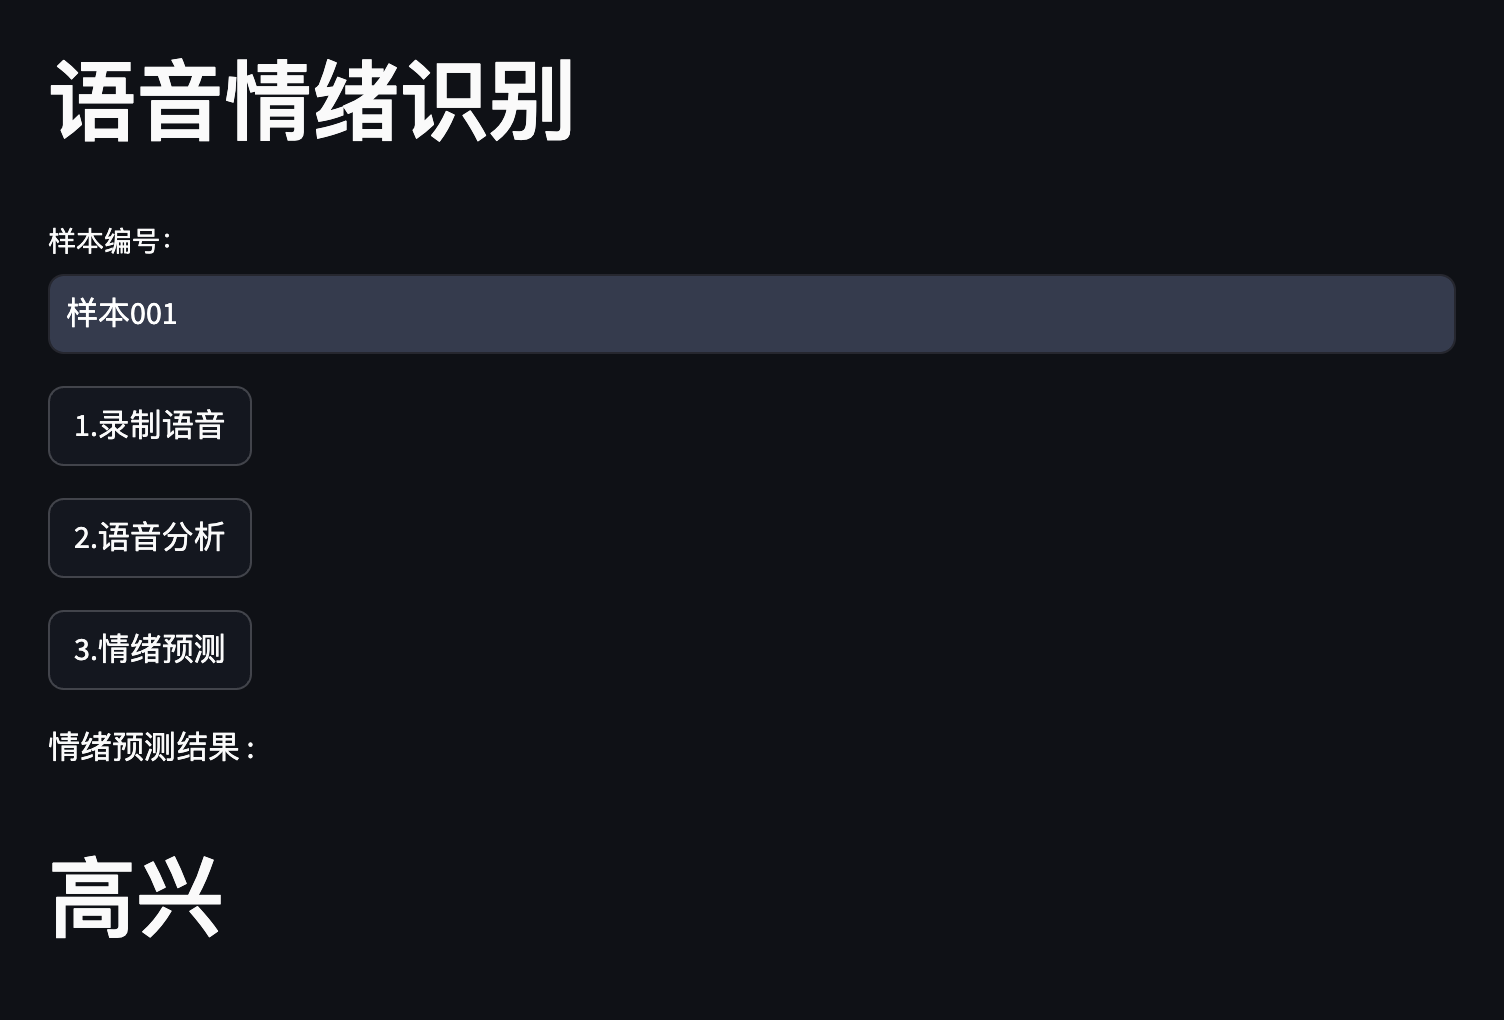
\includegraphics[width=\textwidth]{image/截图5.png}
	\caption{情绪识别}
\end{figure}

\chapter{特征数据}

\section{音频特征}

软件使用librosa库实现了音频数据的分析,Librosa 是一个功能强大且灵活的音频处理库,它提供了丰富的工具和函数,能够满足从音频加载、特征提取、变换到可视化的各种需求。通过 Librosa,开发者可以轻松地进行复杂的音频分析和处理任务。

\subsection{音频特征提取}

\begin{enumerate}
  \item 时域特征
  \begin{enumerate}
  \item librosa.feature.zero\_crossing\_rate:计算过零率(zero-crossing rate)。
  \item librosa.feature.rmse:计算根均方能量(root-mean-square energy)。
\end{enumerate}

  \item 频域特征
  \begin{enumerate}
  \item librosa.feature.mfcc:提取梅尔频率倒谱系数(MFCC)。
  \item librosa.feature.spectral\_centroid:计算谱质心(spectral centroid)。
  \item librosa.feature.spectral\_bandwidth:计算谱带宽(spectral bandwidth)。
  \item librosa.feature.chroma\_stft:计算色度特征(chroma features)。

	\end{enumerate}

\end{enumerate}


\subsection{变换与滤波}

\begin{enumerate}
  \item 短时傅里叶变换(STFT):librosa.stft
  \item 梅尔频谱:librosa.feature.melspectrogram
  \item 倒谱变换:librosa.feature.mfcc
\end{enumerate}

\subsection{音频可视化}

\begin{enumerate}
  \item 波形图:librosa.display.waveplot
  \item 谱图:librosa.display.specshow
  \item 色度图:librosa.display.specshow
\end{enumerate}

\subsection{音高估计和音频时间拉伸}

\begin{enumerate}
  \item librosa.pyin:估计音高
  \item librosa.effects.time\_stretch:时间拉伸。
  \item librosa.effects.pitch\_shift:音高偏移。
\end{enumerate}

\section{语音情绪识别技术}

语音情绪识别(Speech Emotion Recognition, SER)是一种通过分析和处理语音信号来识别说话者情绪状态的技术。它在人机交互、心理健康监测、客服系统等领域有着广泛的应用。以下是对语音情绪识别的详细介绍:
\subsection{基础概念}

语音情绪识别的目标是通过分析语音信号中的特征,判断说话者的情绪状态。常见的情绪分类包括高兴、愤怒、悲伤、惊讶、厌恶、恐惧和中性等。

\subsection{语音情绪识别流程}

语音情绪识别一般包括以下几个步骤:

1.	音频采集:通过麦克风或其他设备采集语音信号。

2.	预处理:对采集到的语音信号进行去噪、归一化等预处理操作,以提高信号质量。

	3.	特征提取:从语音信号中提取能够反映情绪特征的参数。
	
	4.	情感分类:使用机器学习或深度学习算法,根据提取的特征进行情感分类。

\subsection{特征提取}

特征提取是语音情绪识别的关键步骤。常用的特征包括:

	•	时域特征:如平均音量、音量变化率等。
	
	•	频域特征:如基频(F0)、频谱质心、频谱带宽等。
	
	•	时频域特征:如梅尔频率倒谱系数(MFCC)、能量谱包络等。
	
	•	高阶特征:如语速、语音节奏等。
	
\subsection{情感分类}

常用的情感分类方法包括:

	•	机器学习方法:如支持向量机(SVM)、K 近邻(KNN)、随机森林(RF)等。
	
	•	深度学习方法:如卷积神经网络(CNN)、循环神经网络(RNN)、长短期记忆网络(LSTM)等。
	
\section{语音情绪识别模型}

近年来,语音情绪识别技术随着深度学习的进步得到了显著提升。最新的基于语音的情绪识别模型通常结合了复杂的神经网络架构,如卷积神经网络(CNN)、循环神经网络(RNN)以及变换器(Transformer)模型。这些模型能够更有效地捕捉语音信号中的情绪特征,提供更高的准确性和鲁棒性。以下是一些最新的基于语音情绪识别的模型及其特点:

\subsection{CNN-RNN 混合模型}

混合模型结合了 CNN 和 RNN 的优势,通常先使用 CNN 提取语音信号的时频特征,然后通过 RNN 捕捉序列中的时间依赖性。这种方法能够更好地处理语音信号的时变特性。

例子:

	•	CNN-LSTM 模型:
	
	
	•	CNN 部分:用于提取局部时频特征,如梅尔频谱或 MFCC。
	
	•	LSTM 部分:用于捕捉语音信号中的长时间依赖关系。
	
\subsection{Transformer 模型}

Transformer 模型在自然语言处理(NLP)中取得了巨大的成功,也被引入语音情绪识别中。它们通过自注意力机制能够更好地捕捉长时间依赖和复杂关系。

例子:

	•	Wav2vec 2.0:
	
	•	由 Facebook AI Research 提出,基于 Transformer 架构。
	
	•	通过自监督学习方法,从未标注的语音数据中预训练模型,再在情绪识别任务上进行微调。


\subsection{预训练和微调}

使用预训练的音频模型(如 Wav2vec 2.0、HuBERT)进行语音情绪识别。预训练模型能够从大量未标注的数据中学习通用的音频特征,然后通过在小规模标注数据上微调,显著提高情绪识别的准确性。

例子:

HuBERT:

	•	由 Facebook AI Research 提出,基于自监督学习的音频表示学习模型。
	
	•	在大量未标注的语音数据上进行预训练,然后在情绪识别任务上微调。
	
\subsection{多模态融合}

结合语音信号和其他模态(如视频、文本)进行情绪识别。多模态融合方法通过同时分析多个数据源,能够提高情绪识别的准确性和鲁棒性。

例子:

	•	语音-视频情绪识别模型:
	
	•	通过融合语音和视频信号,结合 CNN 处理视频特征,RNN 或 Transformer 处理语音特征,实现情绪识别。
	
\subsection{总结}

最新的语音情绪识别模型结合了先进的深度学习技术,能够更有效地捕捉语音信号中的情绪特征。通过混合模型、Transformer 模型、预训练和微调、多模态融合等方法,语音情绪识别的准确性和鲁棒性得到了显著提升。这些技术的进步为更自然、更智能的人机交互奠定了基础,并在心理健康监测、客服系统等领域具有广泛的应用前景。

\end{document}
